\chapter{Méthodes du gradient conjugué}

Dans ce chapitre, nous présentons les \emph{méthodes du gradient conjugué},
qui constituent une famille d’algorithmes très efficaces pour résoudre
des problèmes quadratiques de grande dimension, ainsi que leurs
extensions non linéaires.

Les méthodes du gradient conjugué ont été introduites dans les années
1950 par Hestenes et Stiefel \cite{hestenes1952methods} pour résoudre des systèmes linéaires
\[
A x = b,
\]
où $A \in \R^{n \times n}$ est symétrique définie positive. Plus tard,
Fletcher et Reeves \cite{fletcher1964function} ont proposé une extension \emph{non linéaire} pour
la minimisation d’une fonction générale $f : \R^n \to \R$.

\medskip

Par rapport à la descente de gradient :
\begin{itemize}
  \item elles ne nécessitent pas de stocker la matrice $A$ ;
  \item elles convergent beaucoup plus rapidement sur les problèmes quadratiques bien conditionnés ;
  \item elles sont particulièrement adaptées aux grandes dimensions.
\end{itemize}

%%%%%%%%%%%%%%%%%%%%%%%%%%%%%%%%%%%%%%%%%%%%%%%%%%%%%%%%%%%%
\section{Gradient conjugué linéaire}

\subsection{Problème quadratique associé}

Considérons le système linéaire
\[
A x = b,
\]
où $A$ est symétrique définie positive. Ce problème est équivalent à la minimisation de
\begin{equation}
q(x) = \frac{1}{2} x^\top A x - b^\top x.
\label{eq:cg-quadratic}
\end{equation}
Son gradient vaut
\[
\nabla q(x) = A x - b,
\]
et donc $x^\star$ minimise $q$ si et seulement si $A x^\star = b$.

Pour une direction $p_k$, on minimise $q(x_k + \alpha p_k)$ :
\[
\psi(\alpha) = q(x_k + \alpha p_k).
\]
La condition $\psi'(\alpha)=0$ donne
\[
p_k^\top A (x_k + \alpha p_k) - p_k^\top b = 0.
\]
Comme $r_k = A x_k - b$ :
\[
\boxed{\alpha_k = -\frac{p_k^\top r_k}{p_k^\top A p_k}}.
\]

%%%%%%%%%%%%%%%%%%%%%%%%%%%%%%%%%%%%%%%%%%%%%%%%%%%%%%%%%%%%
\subsection{Directions \texorpdfstring{$A$}{A}-conjuguées}

\begin{definition}
Deux vecteurs $p_i,p_j$ non nuls sont \emph{$A$-conjugués} si
\[
p_i^\top A p_j = 0.
\]
Une famille $(p_0,\dots,p_m)$ est $A$-conjuguée si tous ses vecteurs sont deux à deux $A$-conjugués.
\end{definition}

Une famille $A$-conjuguée constitue une base dans laquelle la minimisation devient indépendante entre composantes : une correction dans une direction ne dégrade pas celles déjà faites.

%%%%%%%%%%%%%%%%%%%%%%%%%%%%%%%%%%%%%%%%%%%%%%%%%%%%%%%%%%%%
\subsection{Méthode des directions conjuguées}

On suppose données des directions $A$-conjuguées $(\eta_0,\dots,\eta_{n-1})$. On pose :
\[
x_{k+1} = x_k + \alpha_k \eta_k, \qquad
\alpha_k = -\frac{\eta_k^\top r_k}{\eta_k^\top A \eta_k}.
\]

\begin{theoreme}[Minimisation sur sous-espaces croissants]
Pour $k \ge 1$ :
\[
r_k^\top \eta_i = 0 \quad (i<k),
\]
et
\[
\boxed{x_k = \arg\min_{x \in x_0 + \mathrm{span}(\eta_0,\dots,\eta_{k-1})} q(x)}.
\]
\end{theoreme}

%%%%%%%%%%%%%%%%%%%%%%%%%%%%%%%%%%%%%%%%%%%%%%%%%%%%%%%%%%%%
\subsection{Algorithme du gradient conjugué linéaire}

On note $r_k = A x_k - b$.

On définit les directions par
\[
p_0 = -r_0,\qquad p_k = -r_k + \beta_k p_{k-1}.
\]
La condition $A$-conjugaison $p_k^\top A p_{k-1}=0$ impose
\[
\boxed{\beta_k = \frac{r_k^\top A p_{k-1}}{p_{k-1}^\top A p_{k-1}}}
\quad\text{(Hestenes–Stiefel \cite{hestenes1952methods} linéaire).}
\]
Dans la pratique, on utilise souvent la forme équivalente
\[
\beta_k = \frac{r_k^\top r_k}{r_{k-1}^\top r_{k-1}}.
\]

\begin{algorithm}[H]
\caption{Version préliminaire du Gradient Conjugué}
\label{alg:cg-preliminary}
Given $x_0$\;
Set $r_0 \leftarrow Ax_0 - b$, $p_0 \leftarrow -r_0$, $k \leftarrow 0$\;
\While{$r_k \neq 0$}{
    $\alpha_k \leftarrow -\dfrac{r_k'p_k}{p_k'Ap_k}$\;
    $x_{k+1} \leftarrow x_k + \alpha_k p_k$\;
    $r_{k+1} \leftarrow Ax_{k+1} - b$\;
    $\beta_{k+1} \leftarrow \dfrac{r_{k+1}'Ap_k}{p_k'Ap_k}$\;
    $p_{k+1} \leftarrow -r_{k+1} + \beta_{k+1}p_k$\;
    $k \leftarrow k + 1$\;
}
\end{algorithm}

\begin{algorithm}[H]
\caption{Gradient Conjugué (version pratique)}
\label{alg:cg-practical}
Given $x_0$\;
Set $r_0 \leftarrow Ax_0 - b$, $p_0 \leftarrow -r_0$, $k \leftarrow 0$\;
\While{$r_k \neq 0$}{
    $\alpha_k \leftarrow \dfrac{r_k'r_k}{p_k'Ap_k}$\;
    $x_{k+1} \leftarrow x_k + \alpha_k p_k$\;
    $r_{k+1} \leftarrow r_k + \alpha_k Ap_k$\;
    $\beta_{k+1} \leftarrow \dfrac{r_{k+1}'r_{k+1}}{r_k'r_k}$\;
    $p_{k+1} \leftarrow -r_{k+1} + \beta_{k+1}p_k$\;
    $k \leftarrow k + 1$\;
}
\end{algorithm}

\begin{remarque}
La version pratique évite de recalculer $Ax_{k+1}$ en utilisant la relation de récurrence $r_{k+1} = r_k + \alpha_k Ap_k$.
De plus, les formules pour $\alpha_k$ et $\beta_{k+1}$ ne nécessitent que des produits scalaires.
\end{remarque}

Les propriétés suivantes sont vérifiées :
\[
r_i^\top r_j = 0, \qquad p_i^\top A p_j = 0 \quad(i\neq j).
\]

%%%%%%%%%%%%%%%%%%%%%%%%%%%%%%%%%%%%%%%%%%%%%%%%%%%%%%%%%%%%
\subsection{Borne d’erreur et conditionnement}

Si $\lambda_{\min}$ et $\lambda_{\max}$ sont les valeurs propres extrêmes de $A$, alors
\[
\frac{\|x_k - x^\star\|_A}{\|x_0 - x^\star\|_A}
\le
2\left(\frac{\sqrt{\kappa(A)} - 1}{\sqrt{\kappa(A)} + 1}\right)^k,
\qquad
\kappa(A)=\frac{\lambda_{\max}}{\lambda_{\min}}.
\]

%%%%%%%%%%%%%%%%%%%%%%%%%%%%%%%%%%%%%%%%%%%%%%%%%%%%%%%%%%%%
\section{Interprétation géométrique}

\subsection{Niveaux d’une fonction quadratique}

Les ensembles de niveau de \eqref{eq:cg-quadratic} sont des ellipses centrées en $x^\star$.  
Le gradient conjugué suit des directions successivement $A$-conjuguées, ce qui permet de ``corriger'' l’erreur dans chacune des directions de manière indépendante.

\begin{figure}[H]
  \centering
  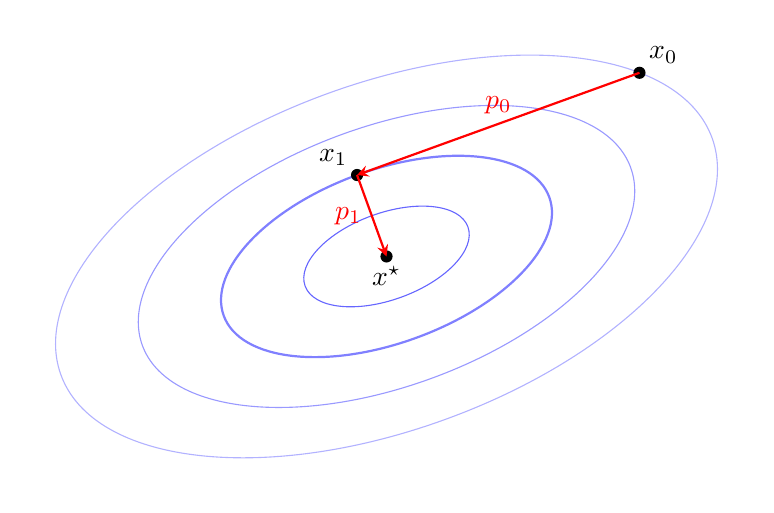
\begin{tikzpicture}[scale=1.1, >=stealth]
    \coordinate (xstar) at (0,0);
    % Level sets (ellipses) - tilted by 20 degrees for consistency with p0 direction
    \begin{scope}[rotate=20]
      \draw[blue!30]       (0,0) ellipse (4 and 2);
      \draw[blue!40]       (0,0) ellipse (3 and 1.5);
      \draw[thick,blue!50] (0,0) ellipse (2 and 1);
      \draw[blue!60]       (0,0) ellipse (1 and 0.5);
    \end{scope}
    
    % x1 on ellipse (2,1) at top of minor axis (s=90°)
    % x = -1*sin(20°) = -0.34, y = 1*cos(20°) = 0.94
    % p1 from x1 to x* will be along minor axis
    \coordinate (x1) at (-0.34, 0.94);
    \fill (x1) circle (2pt) node[above left] {$x_1$};
    
    % x0 on outer ellipse (4,2) at t=30°, positioned so p0 is parallel to major axis
    % x = 4*cos(30°)*cos(20°) - 2*sin(30°)*sin(20°) = 2.92
    % y = 4*cos(30°)*sin(20°) + 2*sin(30°)*cos(20°) = 2.12
    % Direction to x1: slope = 1.18/3.26 ≈ 0.36 = tan(20°) ✓
    \coordinate (x0) at (2.92, 2.12);
    \fill (x0) circle (2pt) node[above right] {$x_0$};
    
    % x* at center
    \fill (xstar) circle (2pt) node[below] {$x^\star$};
    
    % Direction p0: from x0 to x1 - parallel to major axis (slope = tan(20°))
    \draw[->, thick, red] (x0) -- (x1) node[midway, above] {$p_0$};
    
    % Direction p1: from x1 to x* - along minor axis
    \draw[->, thick, red] (x1) -- (xstar) node[midway, left] {$p_1$};
  \end{tikzpicture}
  \caption{Interprétation géométrique : niveaux de $q$ et directions conjuguées.}
\end{figure}

En dimension deux, le gradient conjugué atteint exactement $x^\star$ en deux itérations.

%%%%%%%%%%%%%%%%%%%%%%%%%%%%%%%%%%%%%%%%%%%%%%%%%%%%%%%%%%%%
\section{Comparaison avec la descente de gradient}

La descente de gradient zigzague sur des ellipses allongées, alors que le gradient conjugué choisit des directions qui ``diagonaliseront'' progressivement la matrice $A$.

%%%%%%%%%%%%%%%%%%%%%%%%%%%%%%%%%%%%%%%%%%%%%%%%%%%%%%%%%%%%
\section{Préconditionnement}

Lorsque $A$ est mal conditionnée, on introduit une matrice SPD $M$
approchant $A$ ou $A^{-1}$.  
On considère le système équivalent :
\[
M^{-1} A x = M^{-1} b.
\]

On introduit $z_k = M^{-1} r_k$.

\begin{algorithm}[H]
\caption{Gradient Conjugué Préconditionné}
\label{alg:pcg}
Given $x_0$, preconditioner $M$\;
Set $r_0 \leftarrow Ax_0 - b$\;
Solve $My_0 = r_0$ for $y_0$\;
Set $p_0 \leftarrow -y_0$, $k \leftarrow 0$\;
\While{$r_k \neq 0$}{
    $\alpha_k \leftarrow \dfrac{r_k'y_k}{p_k'Ap_k}$\;
    $x_{k+1} \leftarrow x_k + \alpha_k p_k$\;
    $r_{k+1} \leftarrow r_k + \alpha_k Ap_k$\;
    Solve $My_{k+1} = r_{k+1}$\;
    $\beta_{k+1} \leftarrow \dfrac{r_{k+1}'y_{k+1}}{r_k'y_k}$\;
    $p_{k+1} \leftarrow -y_{k+1} + \beta_{k+1}p_k$\;
    $k \leftarrow k + 1$\;
}
\end{algorithm}
%%%%%%%%%%%%%%%%%%%%%%%%%%%%%%%%%%%%%%%%%%%%%%%%%%%%%%%%%%%%
\section{Gradient conjugué non linéaire}

On cherche à minimiser $f(x)$, supposée $\mathcal{C}^1$.  
On note $g_k = \nabla f(x_k)$.

\begin{algorithm}[H]
\caption{Méthode de Fletcher-Reeves}
\label{alg:fletcher-reeves}
Given $x_0$\;
Evaluate $f_0 = f(x_0)$, $\nabla f_0 = \nabla f(x_0)$\;
Set $p_0 = -\nabla f_0$, $k \leftarrow 0$\;
\While{$\nabla f_k \neq 0$}{
    Compute $\alpha_k$ and set $x_{k+1} = x_k + \alpha_k p_k$\;
    Evaluate $\nabla f_{k+1}$\;
    $\beta_{k+1}^{FR} \leftarrow \dfrac{\nabla f_{k+1}'\nabla f_{k+1}}{\nabla f_k'\nabla f_k}$\;
    $p_{k+1} \leftarrow -\nabla f_{k+1} + \beta_{k+1}^{FR}p_k$\;
    $k \leftarrow k + 1$\;
}
\end{algorithm}

\begin{theoreme}
Si la recherche linéaire satisfait les conditions de Wolfe et si $f$ est régulière, alors
\[
\liminf_{k\to\infty} \|g_k\| = 0.
\]
\end{theoreme}

%%%%%%%%%%%%%%%%%%%%%%%%%%%%%%%%%%%%%%%%%%%%%%%%%%%%%%%%%%%%
\section{Résumé}

\begin{itemize}
  \item Le gradient conjugué linéaire est optimal pour les problèmes quadratiques SPD.
  \item Les directions sont $A$-conjuguées et les résidus orthogonaux.
  \item Le préconditionnement améliore considérablement la convergence.
  \item Le gradient conjugué non linéaire est efficace et peu coûteux.
  \item Le choix de $\beta_k$ influence fortement la performance.
\end{itemize}

%%%%%%%%%%%%%%%%%%%%%%%%%%%%%%%%%%%%%%%%%%%%%%%%%%%%%%%%%%%%
\subsection{Propriétés des itérés et sous-espaces de Krylov}

Les propriétés suivantes justifient l'efficacité théorique de la méthode.

\begin{theoreme}
Supposons que le $k$-ème itéré n'est pas égal à la solution $x^\star$. Alors :
\begin{enumerate}
    \item[(i)] Les résidus sont orthogonaux :
    \[ \forall i = 0, \dots, k-1, \quad r_k^\top r_i = 0. \]
    
    \item[(ii)] L'espace engendré par les résidus est un sous-espace de Krylov de degré $k$ pour $r_0$ :
    \[ \mathrm{span}(r_0, \dots, r_k) = \mathrm{span}(r_0, A r_0, \dots, A^k r_0). \]
    
    \item[(iii)] L'espace engendré par les directions de descente coïncide avec cet espace :
    \[ \mathrm{span}(p_0, \dots, p_k) = \mathrm{span}(r_0, A r_0, \dots, A^k r_0). \]
    
    \item[(iv)] Les directions sont $A$-conjuguées par rapport aux précédentes :
    \[ \forall i = 0, \dots, k-1, \quad p_k^\top A p_i = 0. \]
\end{enumerate}
\end{theoreme}

\begin{proof}[Preuve]
Référence : \cite{nocedal2006numerical}.
\end{proof}

\paragraph{Conséquences.}
D'après le point (iv), le gradient conjugué converge vers $x^\star$ en au plus $n$ itérations (en arithmétique exacte), car il ne peut y avoir plus de $n$ directions non nulles mutuellement $A$-conjuguées dans $\R^n$.

\begin{remarque}
Il est essentiel pour ces propriétés que l'initialisation soit $p_0 = -r_0 = -(A x_0 - b)$.
\end{remarque}

%%%%%%%%%%%%%%%%%%%%%%%%%%%%%%%%%%%%%%%%%%%%%%%%%%%%%%%%%%%%
\subsection{Dérivation de la version efficace (Standard CG)}
\label{sec:efficient-cg}

Jusqu'à présent, nous avions la formule générale pour $\alpha_k$. Nous pouvons la simplifier pour réduire le coût de calcul.

On sait que :
\[ \alpha_k = \frac{-r_k^\top p_k}{p_k^\top A p_k}. \]
D'après le théorème de minimisation sur sous-espace (ESM), on sait que $r_k^\top p_i = 0$ pour tout $i = 0, \dots, k-1$.
Comme $p_k = -r_k + \beta_k p_{k-1}$, on a :
\[ 
-r_k^\top p_k = -r_k^\top (-r_k + \beta_k p_{k-1}) = r_k^\top r_k - \beta_k \underbrace{r_k^\top p_{k-1}}_{=0}.
\]
Ainsi, la formule simplifiée pour le pas est :
\[
\boxed{\alpha_k = \frac{r_k^\top r_k}{p_k^\top A p_k}}.
\]

Ensuite, pour le coefficient $\beta_{k+1}$, nous partons de la définition assurant la $A$-conjugaison :
\[
\beta_{k+1} = \frac{r_{k+1}^\top A p_k}{p_k^\top A p_k}.
\]
Nous utilisons la relation de récurrence du résidu : $r_{k+1} = r_k + \alpha_k A p_k$, ce qui implique $A p_k = \frac{1}{\alpha_k}(r_{k+1} - r_k)$.

En substituant dans le numérateur :
\[
r_{k+1}^\top A p_k = \frac{1}{\alpha_k} r_{k+1}^\top (r_{k+1} - r_k) = \frac{1}{\alpha_k} (r_{k+1}^\top r_{k+1} - \underbrace{r_{k+1}^\top r_k}_{=0}) = \frac{r_{k+1}^\top r_{k+1}}{\alpha_k}.
\]
De même pour le dénominateur, on sait que $p_k^\top A p_k = \frac{r_k^\top r_k}{\alpha_k}$.

Ainsi, le rapport se simplifie remarquablement :
\[
\beta_{k+1} = \frac{\frac{r_{k+1}^\top r_{k+1}}{\alpha_k}}{\frac{r_k^\top r_k}{\alpha_k}} = \frac{r_{k+1}^\top r_{k+1}}{r_k^\top r_k}.
\]

\paragraph{Remarques sur l'Algorithme 7 (Standard CG) :}
\begin{itemize}
    \item Nous avons éliminé les produits matrice-vecteur dans le calcul des coefficients scalaires (ils ne restent que dans la mise à jour $Ap_k$).
    \item Nous n'avons besoin de stocker les valeurs de $x$, $p$ et $r$ que sur deux itérations.
\end{itemize}

%%%%%%%%%%%%%%%%%%%%%%%%%%%%%%%%%%%%%%%%%%%%%%%%%%%%%%%%%%%%
\section{Vitesse de convergence}

\begin{theoreme}[\cite{nocedal2006numerical}]
Si la matrice $A$ possède seulement $r$ valeurs propres distinctes, alors la convergence se produit en au plus $r$ itérations.
\end{theoreme}

Une borne plus précise de l'erreur est donnée par le théorème suivant, qui dépend de la distribution des valeurs propres.

\begin{theoreme}[\cite{luenberger1984linear}]
Si $A$ a pour valeurs propres $\lambda_1 \le \dots \le \lambda_n$, alors :
\[
\| x_{k+1} - x^\star \|_A^2 \le \left( \frac{\lambda_{n-k} - \lambda_1}{\lambda_{n-k} + \lambda_1} \right)^2 \| x_0 - x^\star \|_A^2.
\]
\end{theoreme}
Ce résultat suggère que le gradient conjugué élimine l'influence des valeurs propres extrêmes au fur et à mesure des itérations.

%%%%%%%%%%%%%%%%%%%%%%%%%%%%%%%%%%%%%%%%%%%%%%%%%%%%%%%%%%%%
\subsection{Illustration : Effet de la distribution des valeurs propres}

Considérons une matrice $A$ possédant 2 « clusters » (groupes) de valeurs propres :
\begin{itemize}
    \item Un grand groupe de $n-m$ valeurs propres proches de $\lambda_1$.
    \item Un petit groupe de $m$ valeurs propres (outliers) situées plus loin.
\end{itemize}

D'après le théorème de Luenberger, après $m$ itérations, on élimine l'influence des $m$ valeurs propres extrêmes. L'erreur à l'étape $m+1$ satisfait alors :
\[
\|x_{m+1} - x^\star\|_A^2 \le \left( \frac{\lambda_{n-m} - \lambda_1}{\lambda_{n-m} + \lambda_1} \right)^2 \|x_0 - x^\star\|_A^2.
\]
Grossièrement, cela signifie que la convergence effective démarre après avoir traité les quelques valeurs propres isolées.

%%%%%%%%%%%%%%%%%%%%%%%%%%%%%%%%%%%%%%%%%%%%%%%%%%%%%%%%%%%%
\subsection{Comparaison des taux de convergence}

Il est instructif de comparer la borne d'erreur du Gradient Conjugué (CG) avec celle de la méthode de la Plus Grande Pente (Steepest Descent, SD).

On note le conditionnement $\kappa(A) = \|A\| \cdot \|A^{-1}\| = \frac{\lambda_n}{\lambda_1}$.

\begin{itemize}
    \item \textbf{Pour le Gradient Conjugué (CG) :}
    \[
    \|x_k - x^\star\|_A \le 2 \left( \frac{\sqrt{\kappa(A)} - 1}{\sqrt{\kappa(A)} + 1} \right)^k \|x_0 - x^\star\|_A.
    \]

    \item \textbf{Pour la Plus Grande Pente (SD) :}
    \[
    \|x_k - x^\star\|_A \le \left( \frac{\kappa(A) - 1}{\kappa(A) + 1} \right)^k \|x_0 - x^\star\|_A.
    \]
\end{itemize}

\begin{remarque}
Lorsque $\kappa(A)$ est grand (problème mal conditionné), le terme $\frac{\kappa(A)-1}{\kappa(A)+1}$ est très proche de 1, ce qui implique une convergence très lente (du "bruit" numérique).
En revanche, le terme avec la racine carrée $\sqrt{\kappa(A)}$ dans le CG est beaucoup plus favorable, assurant une convergence plus rapide.
\end{remarque}

%%%%%%%%%%%%%%%%%%%%%%%%%%%%%%%%%%%%%%%%%%%%%%%%%%%%%%%%%%%%
\section{Préconditionnement}
\label{sec:preconditioning}

\subsection{Idée générale}

L'idée du préconditionnement est de « transformer » la distribution des valeurs propres de $A$ pour accélérer la convergence.

Nous effectuons un changement de variable de $x$ vers $\hat{x}$ :
\[
\hat{x} = C x \iff x = C^{-1} \hat{x},
\]
où $C$ est une matrice inversible (non-singulière).

La fonction objective quadratique $\phi(x)$ devient alors une fonction de $\hat{x}$, notée $\hat{\phi}(\hat{x})$ :
\[
\hat{\phi}(\hat{x}) = \phi(C^{-1}\hat{x}) = \frac{1}{2} (C^{-1}\hat{x})^\top A (C^{-1}\hat{x}) - b^\top (C^{-1}\hat{x}).
\]

En développant, on obtient :
\[
\hat{\phi}(\hat{x}) = \frac{1}{2} \hat{x}^\top \left[ (C^{-1})^\top A C^{-1} \right] \hat{x} - \left( (C^{-1})^\top b \right)^\top \hat{x}.
\]

\subsection{Choix de la matrice de préconditionnement}

La fonction $\hat{\phi}$ est toujours quadratique. Si nous utilisons le Gradient Conjugué pour minimiser $\hat{\phi}$, la performance dépendra désormais des valeurs propres de la nouvelle matrice coefficient :
\[
\hat{A} = (C^{-1})^\top A C^{-1}.
\]

Il faut donc choisir la matrice $C$ telle que :
\begin{enumerate}
    \item Le conditionnement de $(C^{-1})^\top A C^{-1}$ soit plus faible que celui de $A$ (c'est-à-dire $\kappa(\hat{A}) < \kappa(A)$).
    \item Ou que les valeurs propres de $(C^{-1})^\top A C^{-1}$ soient bien groupées (clustered).
\end{enumerate}

Dans la pratique, on ne forme pas explicitement $\hat{A}$. On pose souvent $M = C^\top C$ (le préconditionneur) et on adapte l'algorithme CG pour résoudre le système $M^{-1} A x = M^{-1} b$ implicitement.

%%%%%%%%%%%%%%%%%%%%%%%%%%%%%%%%%%%%%%%%%%%%%%%%%%%%%%%%%%%%
\subsection{Mise en œuvre pratique}

En pratique, nous n'avons besoin d'utiliser la matrice $C$ qu'à travers le préconditionneur $M$ défini par :
\[
M = C^\top C.
\]
Ceci mène à l'Algorithme 8 (Gradient Conjugué Préconditionné).

\paragraph{Bilan (Balance).}
L'utilisation du préconditionnement implique un compromis :
\begin{itemize}
    \item[(+)] Le préconditionnement améliore la distribution des valeurs propres (réduisant le nombre d'itérations).
    \item[(-)] Il introduit des résolutions de systèmes linéaires $M y = r$ à chaque étape.
\end{itemize}
Le but est donc de choisir $M$ pour que le système $M y = r$ soit peu coûteux à résoudre.

%%%%%%%%%%%%%%%%%%%%%%%%%%%%%%%%%%%%%%%%%%%%%%%%%%%%%%%%%%%%
\subsection{Exemple : Préconditionnement de Cholesky Incomplet}

Une méthode classique repose sur la décomposition de Cholesky. Pour une matrice $A$ symétrique définie positive, il existe une matrice triangulaire inférieure $L$ telle que $A = L L^\top$.

\textbf{Idée :} On cherche une approximation de $L$ par une matrice \emph{creuse} (sparse) $\tilde{L}$ telle que :
\[
A \approx \tilde{L} \tilde{L}^\top.
\]
On choisit alors $C = \tilde{L}^\top$.
Le préconditionneur devient $M = (\tilde{L}^\top)^\top \tilde{L}^\top = \tilde{L} \tilde{L}^\top$.

La matrice du système transformé est alors :
\[
(C^{-1})^\top A C^{-1} = \tilde{L}^{-1} A (\tilde{L}^{-1})^\top \approx I.
\]
La distribution des valeurs propres de cette matrice est généralement favorable.

\paragraph{Résolution du système.}
Avec ce choix, résoudre $M y = r$ revient à résoudre $\tilde{L} \tilde{L}^\top y = r$. Cela s'effectue par deux résolutions de systèmes triangulaires consécutives (très rapides) :
\begin{enumerate}
    \item Résoudre $\tilde{L} z = r$ pour trouver $z$ (descente).
    \item Résoudre $\tilde{L}^\top y = z$ pour trouver $y$ (remontée).
\end{enumerate}


Voir \cite{langrene2025fast} pour plus de détails.


%%%%%%%%%%%%%%%%%%%%%%%%%%%%%%%%%%%%%%%%%%%%%%%%%%%%%%%%%%%%
